\documentclass{edm_template}

%\usepackage{amsthm,amsmath,amsfonts}
\usepackage{bm}
\usepackage{comment}

\newcommand{\yti}{y_{Ti}}
\newcommand{\yci}{y_{Ci}}
\newcommand{\yhati}{\hat{y}_{Ci}}
\newcommand{\yhat}{\hat{y}_C}
\newcommand{\tauhat}{\hat{\tau}}
\newcommand{\rebar}{\hat{\tau}_{rebar}}
\newcommand{\model}[1]{\hat{y}_C(#1)}
\newcommand{\EE}{\mathbb{E}}

\newtheorem{prop}{Proposition}


\begin{document}

\title{Using Big Data to Sharpen Design-Based Inference in A/B Tests}

\numberofauthors{4} 
\author{
% 1st. author
\alignauthor Anthony Botelho\\
       \affaddr{Worcester Polytechnic Institute}
       \affaddr{100 Institute Rd}\\
       \affaddr{Worcester, MA 01609}\\
       \email{abotelho@wpi.edu}
% 2nd. author
\alignauthor Adam C Sales\\
       \affaddr{University of Texas at Austin}\\
       \affaddr{536C George I. S\'{a}nchez Building}\\
       \affaddr{Austin, TX 78705}\\
       \email{asales@utexas.edu}
% 3rd. author
\alignauthor Thanaporn Patikorn\\
\affaddr{Worcester Polytechnic Institute}
       \affaddr{100 Institute Rd}\\
       \affaddr{Worcester, MA 01609}\\
       \email{tpatikorn@wpi.edu}
\and  % use '\and' if you need 'another row' of author names
% 4th. author
\alignauthor Neil T. Heffernan\\
\affaddr{Worcester Polytechnic Institute}
       \affaddr{100 Institute Rd}\\
       \affaddr{Worcester, MA 01609}\\
       \email{nth@wpi.edu}
}

\maketitle
\begin{abstract}
Randomized A/B tests in educational software are not run in a vacuum: often, reams of historical data are available alongside the data from a randomized trial. This paper proposes a method to use this historical data--often high-dimensional and longitudinal--to improve causal estimates from A/B tests. The method proceeds in two steps: first, fit a machine learning model to the historical data predicting students' outcomes as a function of their covariates. Then, use that model to predict the outcomes of the randomized students in the A/B test. Finally, use design-based methods to estimate the treatment effect in the A/B test, using prediction errors in place of outcomes. This method retains all of the advantages of design-based inference, while, under certain conditions, yielding more precise estimators. This paper will give a theoretical condition under which the method improves precision, and demonstrates it using a deep learning algorithm to help estimate effects in a set of experiments run inside ASSISTments.
\end{abstract}

\section{Introduction}
(Adam)

\section{Data: 22 Experiments and More}
(March and Anthony)

\section{Rebar}
\subsection{Average Treatment Effects in Experiments}
The effect of an intervention $Z$ on an outcome $Y$ is a matter of counterfactuals: how would $Y$ have been different had $Z$ been different? 
To formalize, following \citeN{neyman} and \citeN{rubin}, let $\yci$ be the value of $Y$ subject $i$ would experience if assigned to the control condition and $\yti$ be the value of $Y$ he or she would experience if assigned to the treatment condition. These are called ``potential outcomes.'' The outcome actually observed, $Y_i=Z_i\yti+(1-Z_i)\yci$, is $\yti$ if $i$ is assigned to treatment and $\yci$ if $i$ is assigned to control.\footnote{This notation implicitly assumes the ``stable unit value treatment assignment'' \cite{sutva}, that treatment assignment is well defined and one subject's treatment assignment does not affect other subjects' outcomes.} The treatment effect for $i$ would be $\tau_i\equiv \yti-\yci$. Since for each subject only one of $\yti$ or $\yci$ is ever actually observed, $\tau_i$ is, in general, unknowable. However, aggregate quantities such as the ``sample average treatment effect'' (ATE), $\bar{y}_T-\bar{y}_C$ may be estimated in experiments. Here, $\bar{y}_T$ is the average potential outcome under treatment for all subjects in the experiment (treatment and control), and $\bar{y}_C$ is the average of $y_C$ for all subjects.

If $Z$ is randomized, then the treatment group is a random sample of all experimental subjects, and $\bar{Y}_{Z=1}$, the average observed outcome for treated subjects, is an unbiased estimate of $\bar{y}_T$, the average of $y_T$ over all subjects and $\bar{Y}_{Z=0}$ unbiasedly estimates $\bar{y}_C$. Then their difference, 
\begin{equation}\label{eq:tauEst}
\tauhat=\bar{Y}_{Z=1}-\bar{Y}_{Z=0}
\end{equation}
is an unbiased estimate of the ATE. 
Perhaps surprisingly, the standard error for $\tauhat$ is not identified; however, a popular conservative bound \cite{neyman} is
\begin{equation}\label{eq:tauSE}
Var(\tauhat)=\frac{S^2(Y_{Z=1})}{n_T}+\frac{S^2(Y_{Z=1})}{n_C}
\end{equation}
where $n_T$ is the number of subjects assigned to treatment, $n_C$ is the number assigned to control, $S^2(Y_{Z=1})$ and $S^2(Y_{Z=0})$ are the sample variances of $Y$ in the treatment and control groups, respectively. 
Note that this discussion assumes nothing about the distribution of $Y$ in either treatment group. 

By regressing $Y$ on $Z$ and a matrix of covariates $\bm{x}$---variables defined prior to treatment assignment---it is often possible to estimate the ATE more precisely---although the wrong functional form or other mistaken assumptions can introduce bias \cite{freedman}.  
When covariates are high-dimensional or complex (e.g. longitudinal), these problems are exacerbated. 
In particular, extensive model selection renders inference from regression all but impossible. 

\subsection{Historical Data and Covariates} 
None of this leaves much room for the remnant from an experiment: subjects who were not randomized, perhaps because their classrooms did not participate or because they were no longer eligible when the experiment began. 
On the one hand, data from the remnant can only confuse matters---treatment was not randomized in the remnant, and the remnant may differ from experimental subjects in all sorts of ways. 
On the other hand, including it in the analysis may increases the sample size dramatically, and increase precision.

In fact, you can have it both ways, using the remnant to increase precision without sacrificing any of the advantages of experimentation. 
This is how:
\begin{enumerate}
 \item Using data from the remnant, train a model $\model{\cdot}$ predicting $y_C$ as a function of $\bm{x}$.
 \item Validate $\model{\cdot}$ (using cross-validation or other techniques). if it performs well, proceed; otherwise return to (1).
 \item Use $\model{\cdot}$ and covariates $\bm{x}$ in the experimental sample to generate predicted outcomes $\model{\bm{x}}$ and residuals, $e=Y-\model{\bm{X}}$.
 \item Estimate the ATE as in (\ref{eq:tauEst}) and (\ref{eq:tauSE}), replacing $e$ for $Y$:
 \begin{equation}\label{eq:rebarEst}
 \rebar=\bar{e}_{Z=1}-\bar{e}_{Z=0}
\end{equation}
and 
\begin{equation}\label{eq:rebarSE}
Var(\rebar)=\frac{S^2(e_{Z=1})}{n_T}+\frac{S^2(e_{Z=1})}{n_C}
\end{equation}
\end{enumerate}
Just like the traditional estimator (\ref{eq:tauEst})-(\ref{eq:tauSE}), the rebar estimator $\rebar$ is design-based---its logical basis is the designed experiment, not a model. 
On the other hand, it harvests information from the remnant to improve upon $\tauhat$.
Since it uses the remnant to extract prediction residuals from the outcome, we call it ``remnant-based residualization", or ``rebar.''

The tool rebar uses is the model $\model{\cdot}$, which predicts $y_C$ as a function of $\bm{x}$. 
In EDM settings, the dimension of available covariates is very large, and sample sizes are often large as well---machine learning algorithms make strong candidates for $\model{\cdot}$.
$\model{\cdot}$ is not a statistical model \emph{per se}, estimating the parameters of a probability distribution, but as a tool for prediction.
Indeed, it need not be correct in any sense, and its estimates need not be unbiased or consistent. 
Since it is fit on a separate sample from the experimental subjects, the process of fitting it---steps 1 and 2 above---do not affect standard errors, and model misspecification does not lead to bias.

Rebar improves the precision of an experimental estimate if the variance of the residuals $\bm{e}$ is less than the variance of the raw outcomes $Y$.
This will be the case if $\model{\bm{X}}$ is a good prediction of $y_C$---by residualizing, we subtract out the component of $Y$'s variance that is predicted by $\model{\bm{x}}$. 
In fact, we will show in our results, below, that the Pearson correlation between $\model{\bm{x}}$ and $Y_{Z=0}$ is a strong predictor of the extent rebar improves upon $\tauhat$. 

The previous discussion assumed simple randomization. 
However, rebar easily extends to more complex designs.
Further, as we will illustrate below, rebar can be extended to regression estimators of causal effects as well, modeling low-dimensional covariates within sample and high-dimensional covariates out of sample. 


\section{Deep Learning to Predict Completion}
(Anthony)

\section{Results}
\begin{figure}
\centering
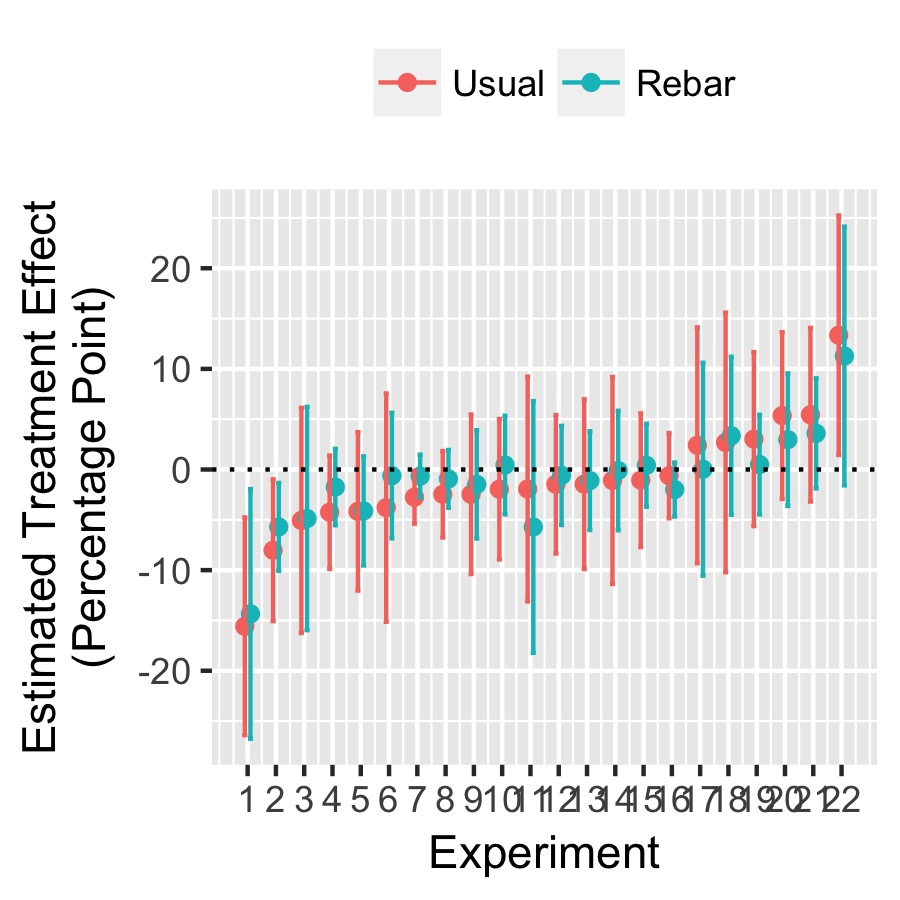
\includegraphics[width=0.5\textwidth]{estEff1.jpg}
\caption{Effect estimates and 95\% confidence intervals for the 22 experiments, using both the usual and rebar estimates. Experiments are ordered by their estimated effect.}
\label{fig:estEff1}
\end{figure}
\begin{figure}
\centering
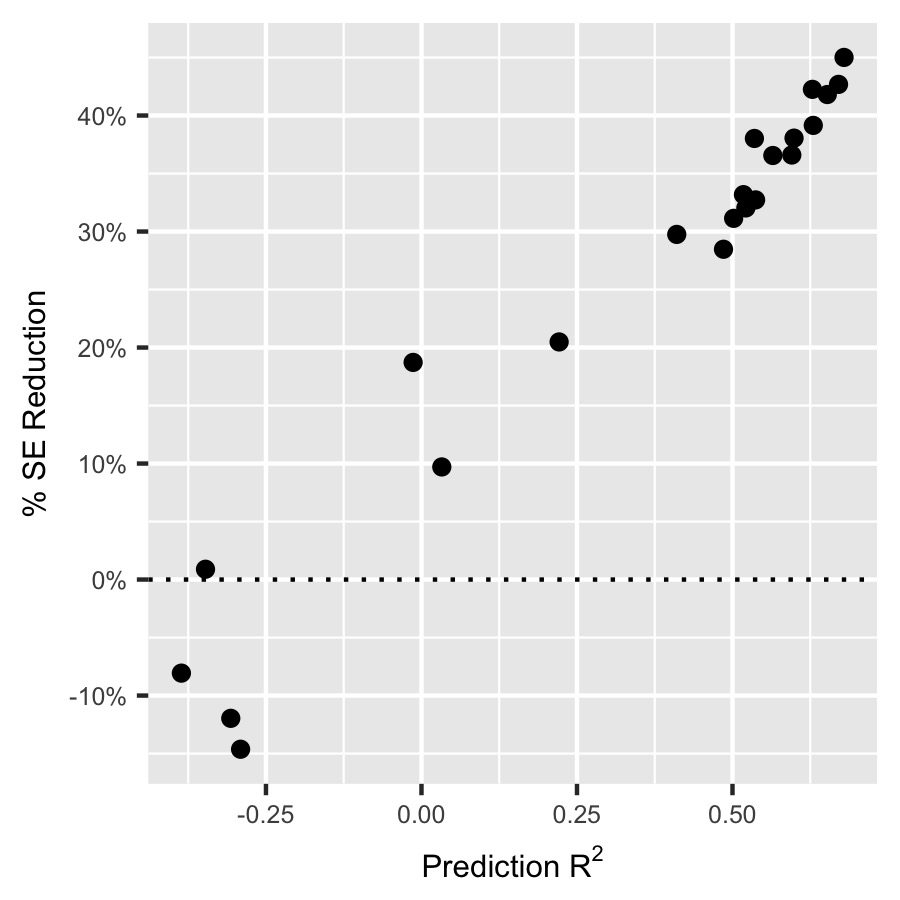
\includegraphics[width=0.5\textwidth]{corVsSE.jpg}
\caption{The improvement in precision of effect estimates, as a percentage of the usual precision estimate, $[SE(\tauhat)-SE(\rebar)]/SE(\tauhat)$ plotted as a function of the correlation of outcomes and predictions, $cor(Y,\model{\bm{x}})$.}
\end{figure}

\begin{comment}
\subsection{Incorporating Regression Controls}
\begin{figure}
\centering
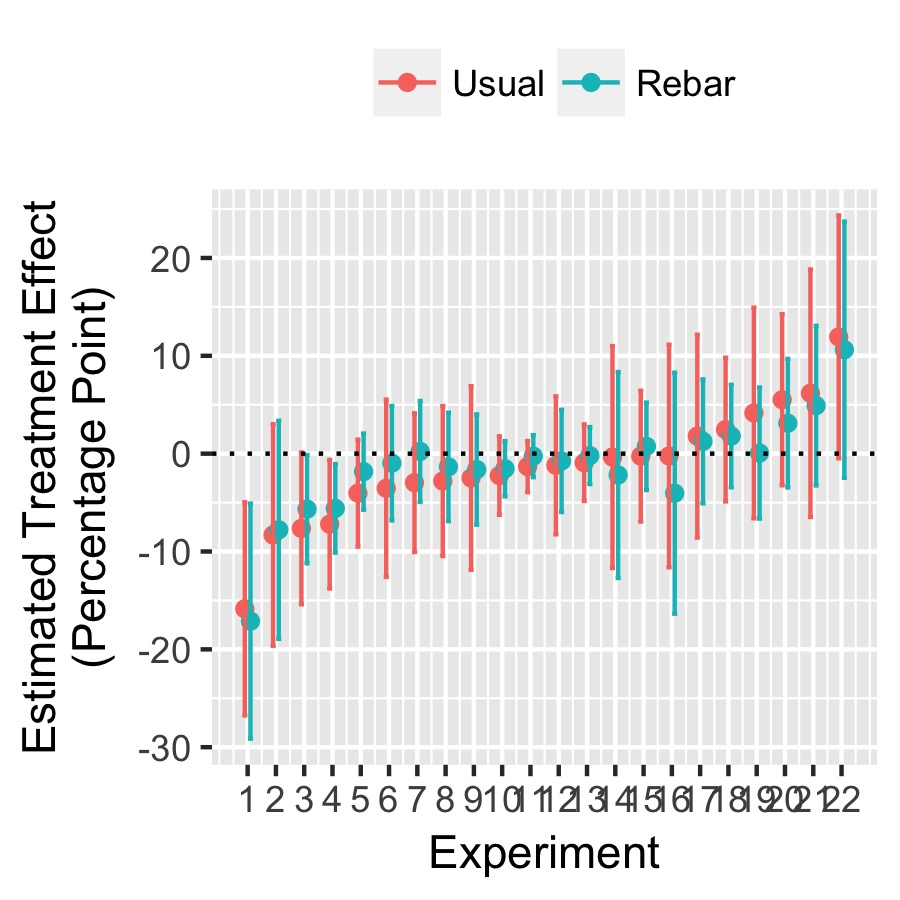
\includegraphics[width=0.5\textwidth]{estEff2.jpg}
\caption{Effect estimates and 95\% confidence intervals for the 22 experiments, from regressions of $Y$ (usual) or $e$ (rebar) on $Z$, prior \% Completed and Prior \% Correct.}
\label{fig:estEff1}
\end{figure}

\begin{figure}
\centering
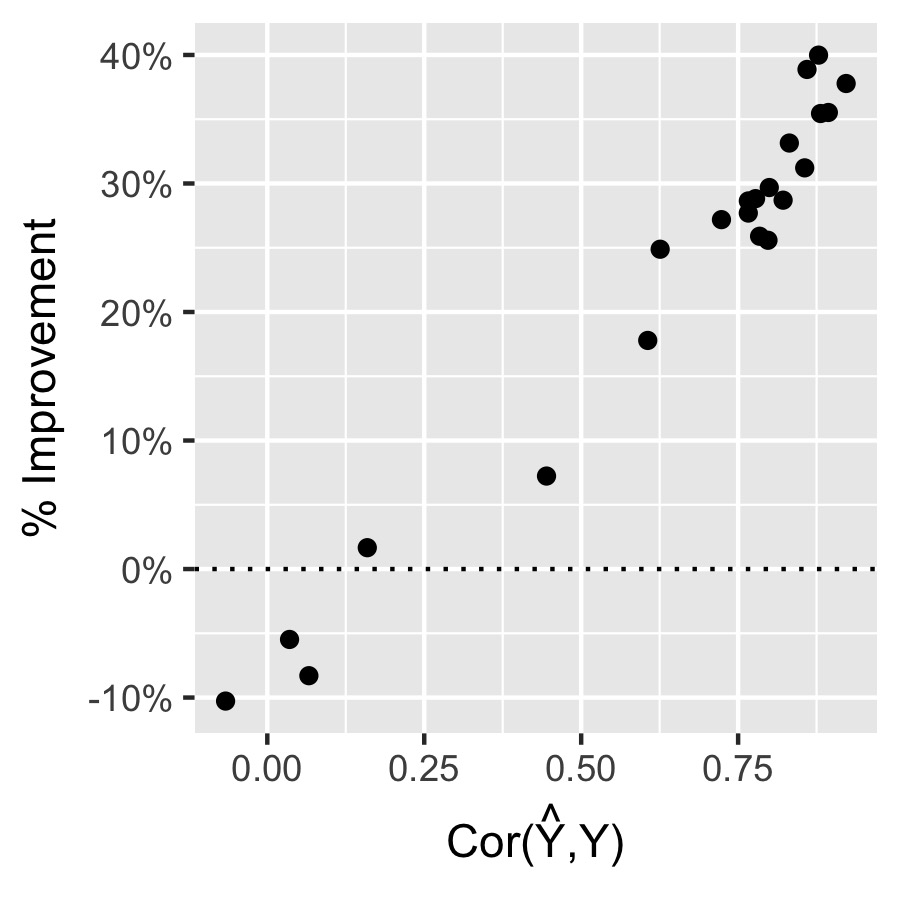
\includegraphics[width=0.5\textwidth]{corVsSE2.jpg}
\caption{The improvement in precision of effect estimates, as a percentage of the usual precision estimate for the usual and rebar regression estimators, plotted as a function of the correlation of outcomes and predictions, $cor(Y,\model{\bm{x}})$.}
\end{figure}
\end{comment}




\section{Discussion}
(Adam)

\bibliographystyle{abbrv}
\bibliography{citations}  
\end{document}
